\documentclass{VUMIFPSkursinis}
\usepackage{algorithmicx}
\usepackage{algorithm}
\usepackage{algpseudocode}
\usepackage{amsfonts}
\usepackage{amsmath}
\usepackage{bm}
\usepackage{caption}
\usepackage{color}
\usepackage{float}
\usepackage{graphicx}
\usepackage{listings}
\usepackage{float}
\usepackage{subfig}
\usepackage{wrapfig}
\usepackage[hidelinks]{hyperref}
\usepackage{todonotes}
\usepackage{xcolor}
% Titulinio aprašas
\university{Vilniaus universitetas}
\faculty{Matematikos ir informatikos fakultetas}
\department{}
\papertype{Programų kūrimo proceso laboratorinis darbas}
\title{Įmonės ,,Mėnuliukų technologijos" programų kūrimo proceso aprašas}
\titleineng{Description of the development process of the ,,Mėnuliukų technologijos" company}
\status{4 kurso 3 grupės studentai}
\author{Mėnuliukai}


\supervisor{Saulius Ragaišis, Doc., Dr.}
\date{Vilnius – \the\year}

% Nustatymai
% \setmainfont{Palemonas}   % Pakeisti teksto šriftą į Palemonas (turi būti įdiegtas sistemoje)
\bibliography{bibliografija}

\begin{document}
\maketitle

\tableofcontents
	\section{Vertinimo apimtis}
		\begin{itemize}
			\item{Vertinta pagal - CMMI-DEV, V1.3}
			\item{Vertinimo apimtis - visa antrame darbe pagerinta organizacija.}
			\item{Aukščiausias vertinamas gebėjimo lygis - maksimalus kurį gali pasiekti procesų sritis.}
			\item{Vertinamos procesų sritys:
				\begin{enumerate}
					\item{Causal Analysis and Resolution}
					\item{Configuration Management}
					\item{Integrated Project Management}
					\item{Organizational Process Definition}
					\item{Organizational Performance Management}
					\item{Organizational Process Performance}
					\item{Project Planning}
					\item{Process and Product Quality Assurance}
					\item{Quantitive Project Management}
					\item{Requirement Development}
					\item{Requirements Management}
					\item{Technical Solution}
					\item{Validation}
					\item{Verification}
				\end{enumerate}
			}
		\end{itemize}
	\section{Vertinimo rezultatai prieš pagerinimą}
	\begin{figure}[!htbp]
		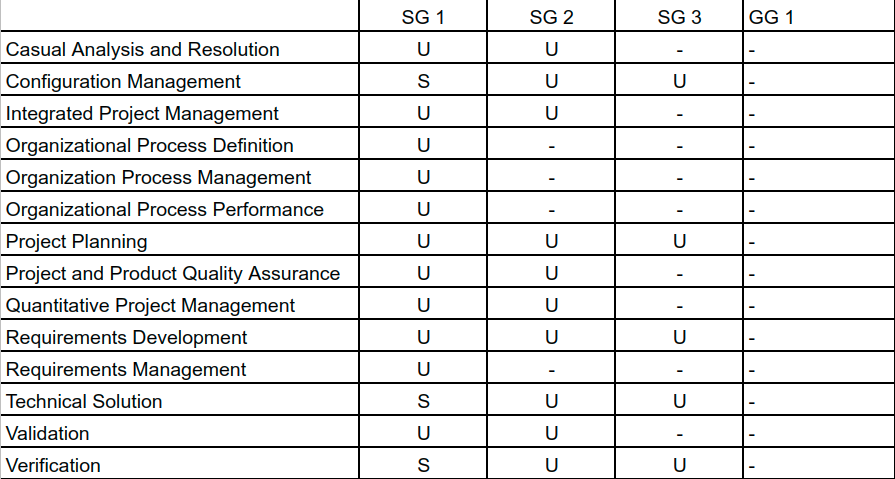
\includegraphics[scale=0.55]{img/profilisPriesLentele}
		\caption{CMMI vertinimo rezultatų gebėjimo profilis prieš pagerinimą lentelėje} % Antraštė įterpiama po paveikslėlio
		\label{img:ProfilisPries}
	\end{figure}
	\begin{figure}[!htbp]
		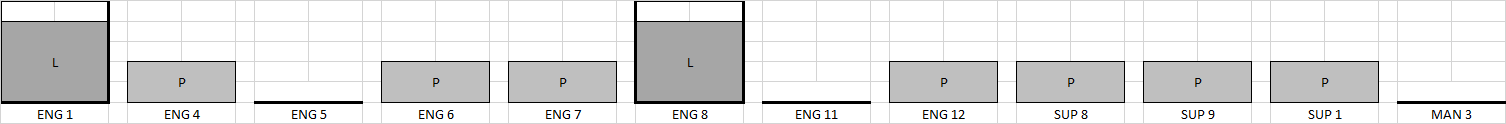
\includegraphics[scale=0.8]{img/ProfilisPries}
		\caption{CMMI vertinimo rezultatų gebėjimo profilis prieš pagerinimą} % Antraštė įterpiama po paveikslėlio
		\label{img:ProfilisPries}
	\end{figure}
	\section{Technical solution}
		\subsection{Pagerinimas}
			\subsubsection{Proceso aprašymas po pagerinimo}
		\subsection{NI PI LI FI atitikimas po pagerinimo}
	\section{Verification}
		Buvo nutarta, kad įmonėje vertifikaciją yra viena iš labiau išvystytų aspektų todėl norėjom jį dar labiau pastumti į priekį, kad ši sritis tarnautų dar ilgą laiką. 
		Taip pat pamanėme, kad jeigu verifikacijos veikla įmonėje būtų išvystyta pilniau, būtų mažiau pataisymų, perdarimų ir konfliktų su užsakovų dėl produkto kuris neatitiktų reikalavimų.
		\subsection{Pagerinimas}
			\subsubsection{Proceso aprašymas po pagerinimo}
		\subsection{NI PI LI FI atitikimas po pagerinimo}
	\section{Configuration management}
	Konfigūracijos valdymas yra vienas svarbiausių procesų norint patikimai kurti programų sistemas, todėl pasirinkome jį tobulinti.
		\subsection{Pagerinimas}
		\begin{itemize}
			\item Pridėtos veiklos standarto išleidimui, pakeitimų dokumentavimui bei auditui.
			\item Pridėtas konfigūracijos pakeitimų prioritizavimas.
		\end{itemize}
			\subsubsection{Proceso aprašymas po pagerinimo}
			\begin{center}
				\begin{table}[ht]
					\caption{Konfigūracijos valdymo procesas}
					\begin{tabular}{ | l | l | }
						\hline
						Pavadinimas:         & Konfigūracijos valdymas.				\\ \hline
						Tikslas:             & \textcolor{black}{Atnaujinti sprinto konfigūraciją.}			\\ \hline
						Vykdytojai:          & \textcolor{black}{devOps specialistai, programuotojai.}			\\ \hline
						Veiklos:             	& \textcolor{blue}{V1 - Pakeitimų validumo užtikrinimas.	}		\\ \hline
																& \textcolor{black}{V2 - Repozitorijos su konfigūracijomis atnaujinimas.}	\\
																 & \textcolor{black}{V3 - Duomenų bazės atnaujinimas.	}		\\ \hline
																 & \textcolor{blue}{V4 - Standarto išleidimas.	}		\\ \hline
																 & \textcolor{blue}{V5 - Konfigūracinių pakeitimų dokumentavimas.	}		\\ \hline
																 & \textcolor{blue}{V6 - Konfigūracijos pakeitimų auditas.	}		\\ \hline
						Naudojami produktai: & \textcolor{black}{NP1 - Konfigūracijos pakeitimų sąrašas.	}	\\ \hline
						Sukuriami produktai: & \textcolor{black}{SP1 - Pamodifikuota konfigūracijų repozitorija. }	\\
																 & \textcolor{black}{SP2 - Atnaujinta duomenų bazė. }			\\ \hline
																 & \textcolor{blue}{SP3 - Konfigūracijos standarto dokumentas. }			\\ \hline
																 & \textcolor{blue}{SP3 - Audito rezultatų dokumentas. }			\\ \hline
																 & \textcolor{blue}{SP4 - Konfigūracinių pakeitimų dokumentas. }			\\ \hline
					\end{tabular}
				\end{table}
			\end{center}
				\textcolor{blue}{Sprinto metu atlikti konfigūracijos pakeitimai yra prioritizuojami pagal jų svarbą, patikrinimas jų validumas, ar jie yra autorizuoti.}\textcolor{black}{Sprinto pabaigoje devOps specialistai peržvelgia atliktus konfigūracinius pakeitimus, kuriuos programuotojai pažymi sprinto metu.
				Šie konfigūracijos pakeitimai yra įdedami į aukštesnę aplinką.} Taip pat po sprinto kodas yra sudedamas į aukštesnę aplinką tolimesniam testavimui.
				\textcolor{blue}{Pagal skirtingus kvalifikacijos lygius programuotojams ar kitiems specialistams suteikiami skirtingi leidimai peržiūrėti/keisti konfigūracijas. Atlikus konfigūracinius pakeitimus sukuriamas dokumentas su konfigūracijos metrikomis, pagal kurį būtų galima atkurti esamą sistemos būseną. Šiam dokumentui priskiriamas unikalus numeris.} \newline
				\textcolor{blue}{Atlikti konfigūraciniai pakeitimai yra detaliai dokumentuojami, yra užtikrinama, kad reikiami asmenys turėtų prieigą prie šių pakeitimų būsenos.} \newline
				\textcolor{blue}{Konfigūracijos pakeitimai taip pat sudedami į tam skirtą duomenų bazę tolimesniam jų sekimui.} \newline
				\textcolor{blue}{Po visų pakeitmų atliekamas auditas norint užtikrinti, ar naujai išleistas standartas yra integralus, ar konfigūraciniai įrašai atitinka konfigūracinius vienetus. Patvirtinamas konfigūracinių vienetų pilnumas, jų nuoseklumas. Radus neatitikimų sukuriamas veiksmų planas jiems išspręsti.}
		\subsection{NI PI LI FI atitikimas po pagerinimo}
		\begin{figure}[!htbp]
			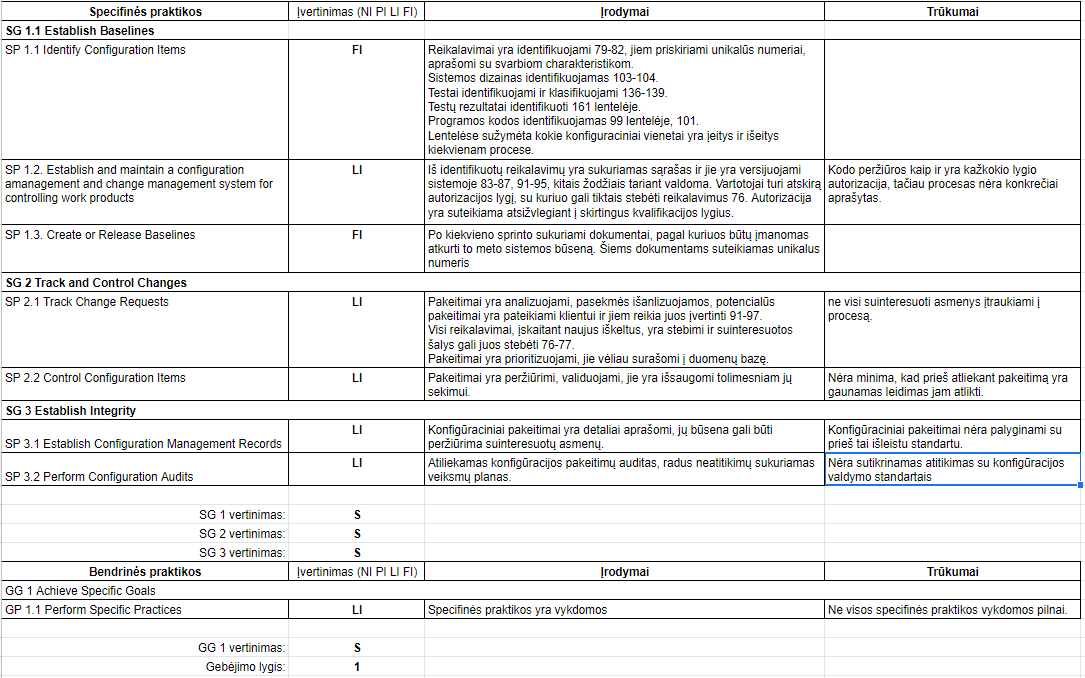
\includegraphics[scale=0.6]{img/konfiguracijosValdymasPataisytas}
			\caption{Konfigūracijos valdymo vertimas po pataisymo} % Antraštė įterpiama po paveikslėlio
			\label{img:ProfilisPo}
		\end{figure}
	\section{Vertinimo rezultatai po pagerinimo}
	\begin{figure}[!htbp]
		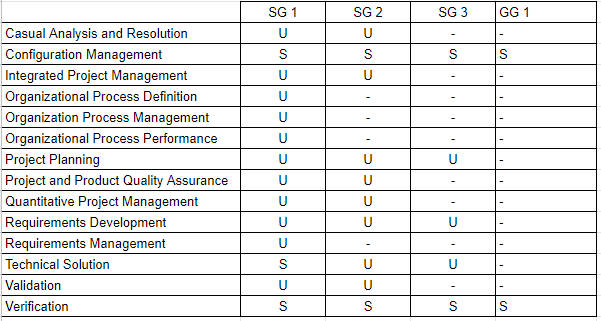
\includegraphics[scale=0.9]{img/poPataisymo}
		\caption{CMMI vertinimo rezultatų gebėjimo profilis po pagerinimo lentelėje} % Antraštė įterpiama po paveikslėlio
		\label{img:ProfilisPo}
	\end{figure}
	\begin{figure}[!htbp]
		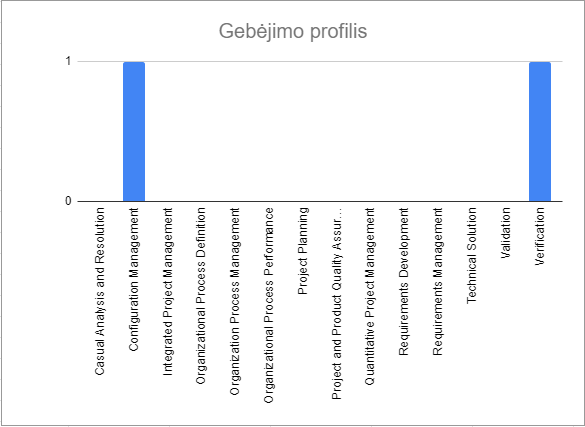
\includegraphics[scale=0.8]{img/poPataisymoProfilis}
		\caption{CMMI vertinimo rezultatų gebėjimo profilis po pagerinimo} % Antraštė įterpiama po paveikslėlio
		\label{img:ProfilisPo}
	\end{figure}

\end{document}
